\subsection{Event-Driven Architecture - EDA}

\subsubsection{Mô tả hệ thống}
Event-Driven Architecture (EDA) là một mô hình kiến trúc phần mềm trong đó các thành phần của hệ thống giao tiếp với nhau thông qua các sự kiện (events). Trong kiến trúc này, các thành phần không tương tác trực tiếp với nhau thông qua các lời gọi hàm hoặc API đồng bộ, mà thay vào đó các thành phần sẽ phát sinh sự kiện khi có thay đổi trạng thái hoặc khi một hành động xảy ra. Các thành phần khác trong hệ thống có thể lắng nghe và phản ứng lại các sự kiện này.

Trong hệ thống IoT, Event-Driven Architecture đặc biệt phù hợp vì các thiết bị IoT thường liên tục tạo ra dữ liệu và các sự kiện từ môi trường. Ví dụ, một cảm biến nhiệt độ có thể tạo ra sự kiện khi nhiệt độ vượt quá một ngưỡng nhất định, hoặc một cảm biến chuyển động có thể phát sinh sự kiện khi phát hiện chuyển động trong khu vực được giám sát. Những sự kiện này sau đó được gửi đến hệ thống xử lý để kích hoạt các hành động tương ứng như gửi cảnh báo, lưu trữ dữ liệu hoặc điều khiển các thiết bị khác.

Một hệ thống EDA điển hình thường bao gồm một số thành phần chính. Thành phần đầu tiên là event producers, tức là các thành phần tạo ra sự kiện. Trong hệ thống IoT, các thiết bị cảm biến và thiết bị thông minh thường đóng vai trò là event producers vì chúng liên tục thu thập dữ liệu từ môi trường và phát sinh các sự kiện khi có thay đổi. Thành phần thứ hai là event broker hoặc event bus, có nhiệm vụ nhận và phân phối các sự kiện đến các thành phần khác trong hệ thống. Event broker đóng vai trò như một trung gian giúp các thành phần trong hệ thống có thể giao tiếp với nhau một cách linh hoạt mà không cần biết trực tiếp về nhau. Thành phần thứ ba là event consumers, tức là các thành phần nhận sự kiện và thực hiện các hành động tương ứng.

Trong nhiều hệ thống IoT hiện đại, các nền tảng xử lý sự kiện thường được triển khai trên các hệ thống phân tán hoặc các nền tảng điện toán đám mây. Các công nghệ như message queue hoặc hệ thống streaming dữ liệu thường được sử dụng để xử lý lượng lớn sự kiện được tạo ra từ các thiết bị IoT. Điều này cho phép hệ thống có thể xử lý dữ liệu theo thời gian thực và mở rộng khi số lượng thiết bị tăng lên.

Một đặc điểm quan trọng của Event-Driven Architecture là tính bất đồng bộ (asynchronous communication). Trong kiến trúc này, các thành phần không cần chờ phản hồi từ các thành phần khác sau khi gửi sự kiện. Điều này giúp giảm sự phụ thuộc giữa các thành phần và giúp hệ thống có thể xử lý nhiều sự kiện cùng lúc. Nhờ đó, EDA đặc biệt phù hợp với các hệ thống IoT có quy mô lớn và yêu cầu xử lý dữ liệu theo thời gian thực.

Ngoài ra, Event-Driven Architecture còn hỗ trợ việc xây dựng các hệ thống có khả năng mở rộng cao. Khi số lượng thiết bị IoT tăng lên, hệ thống có thể dễ dàng bổ sung thêm các thành phần xử lý sự kiện mà không cần thay đổi các thành phần hiện có. Điều này giúp hệ thống có thể thích nghi với sự phát triển nhanh chóng của các ứng dụng IoT.
Sơ đồ kiến trúc
\begin{figure}[H]
    \centering
    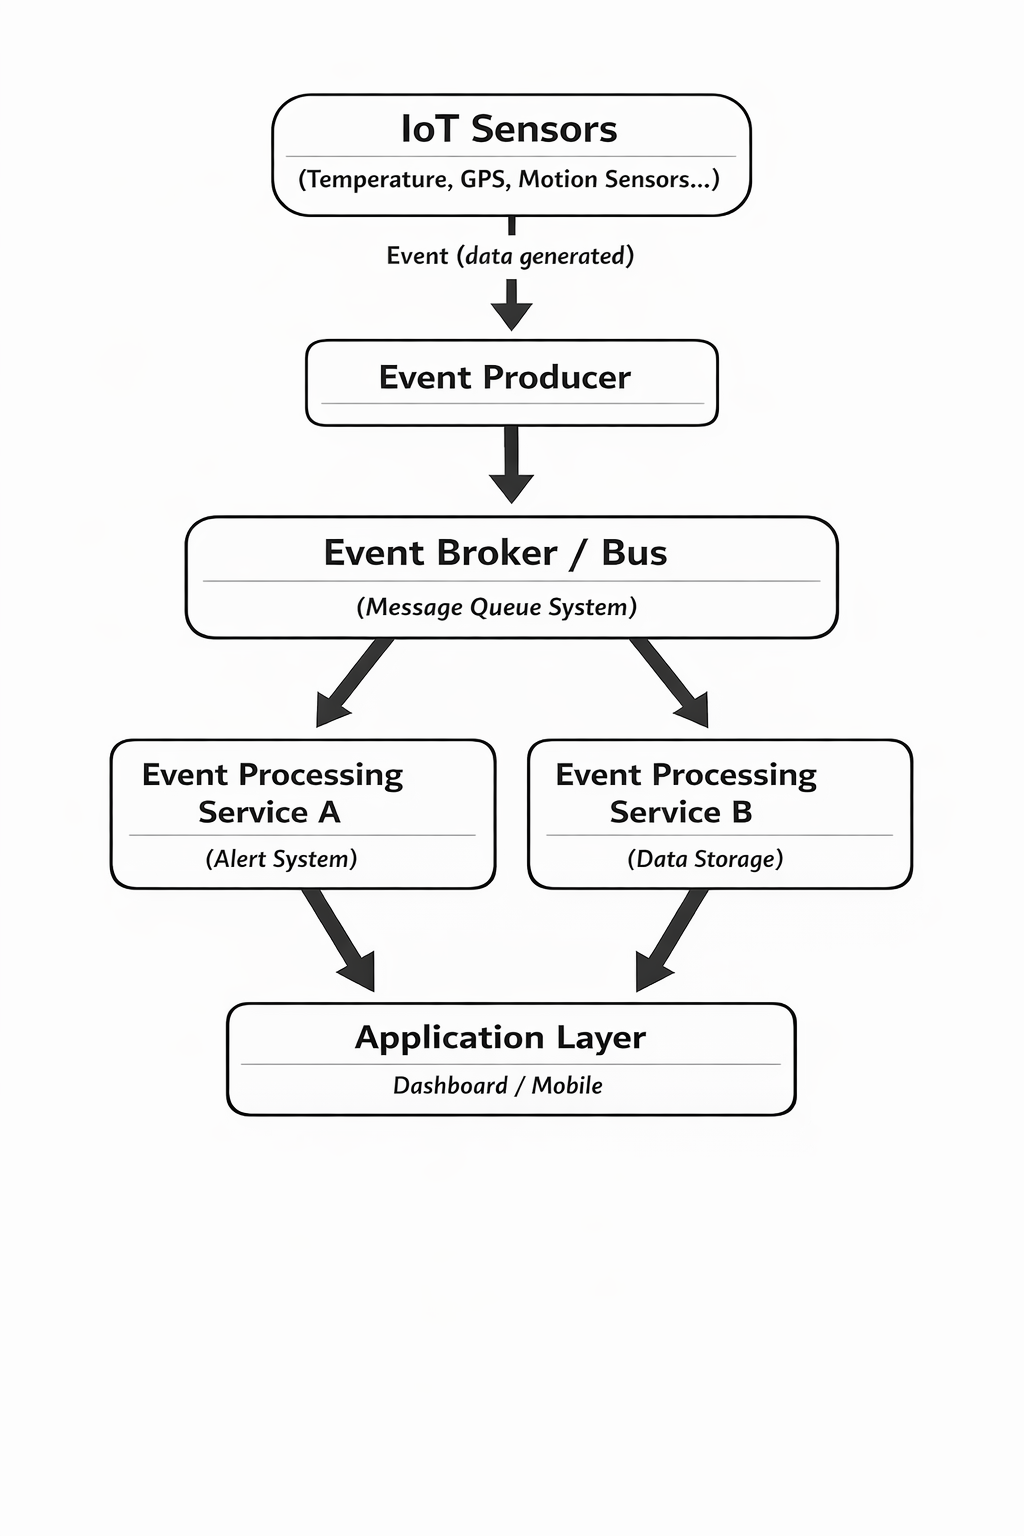
\includegraphics[width=0.5\linewidth]{graphics/EDA Architecture.png}
    \caption{Kiến trúc Event-Driven Architecture}
    \label{fig:placeholder}
\end{figure}

\subsubsection{Phân tích sự đánh đổi}

Mặc dù Event-Driven Architecture mang lại nhiều lợi ích cho các hệ thống IoT, việc áp dụng kiến trúc này cũng đi kèm với một số sự đánh đổi quan trọng. Việc hiểu rõ những trade-off này giúp các kiến trúc sư phần mềm có thể đưa ra quyết định phù hợp khi thiết kế hệ thống.

Một trong những lợi ích lớn nhất của Event-Driven Architecture là khả năng mở rộng (scalability). Do các thành phần trong hệ thống được tách rời và giao tiếp thông qua các sự kiện, hệ thống có thể dễ dàng mở rộng bằng cách thêm các thành phần xử lý sự kiện mới. Tuy nhiên, điều này cũng có thể làm tăng độ phức tạp của hệ thống, đặc biệt khi số lượng sự kiện và thành phần xử lý trở nên rất lớn. Việc theo dõi luồng dữ liệu và xác định nguyên nhân của các lỗi trong hệ thống có thể trở nên khó khăn hơn.

Một trade-off khác liên quan đến tính nhất quán dữ liệu (data consistency). Trong các hệ thống sử dụng Event-Driven Architecture, dữ liệu thường được xử lý theo mô hình bất đồng bộ. Điều này có thể dẫn đến tình trạng dữ liệu trong các thành phần khác nhau của hệ thống không được cập nhật ngay lập tức. Thay vì đạt được tính nhất quán tức thời, hệ thống thường áp dụng mô hình eventual consistency, trong đó dữ liệu sẽ trở nên nhất quán sau một khoảng thời gian nhất định.

Ngoài ra, Event-Driven Architecture cũng có thể tạo ra những thách thức trong việc quản lý và giám sát hệ thống. Khi các thành phần giao tiếp thông qua các sự kiện, việc theo dõi dòng chảy của dữ liệu và xác định vị trí xảy ra lỗi có thể trở nên khó khăn. Do đó, các hệ thống EDA thường cần các công cụ giám sát và logging mạnh mẽ để giúp phát hiện và xử lý sự cố.

Một yếu tố khác cần xem xét là độ trễ (latency) trong hệ thống. Trong một số trường hợp, việc xử lý sự kiện thông qua nhiều thành phần trung gian có thể làm tăng độ trễ của hệ thống. Điều này có thể ảnh hưởng đến các ứng dụng yêu cầu phản hồi nhanh. Vì vậy, khi thiết kế hệ thống EDA cho IoT, cần cân nhắc giữa lợi ích của kiến trúc bất đồng bộ và yêu cầu về hiệu suất của ứng dụng.

\begin{table}[h]
\centering
\caption{Trade-off của Event-Driven Architecture trong hệ thống IoT}
\begin{tabular}{|p{3.5cm}|p{6cm}|p{5.5cm}|}
\hline
\textbf{Tiêu chí} & \textbf{Ưu điểm} & \textbf{Nhược điểm} \\ \hline

Khả năng mở rộng (Scalability) 
& Hệ thống dễ mở rộng vì các dịch vụ hoạt động độc lập 
& Khi số lượng sự kiện quá lớn, cần hạ tầng mạnh để xử lý \\ \hline

Tính linh hoạt (Flexibility) 
& Có thể thêm hoặc thay đổi các dịch vụ xử lý sự kiện mà không ảnh hưởng hệ thống 
& Thiết kế hệ thống ban đầu phức tạp hơn \\ \hline

Khả năng phản ứng thời gian thực 
& Hệ thống có thể phản ứng nhanh với các sự kiện từ thiết bị IoT 
& Có thể phát sinh độ trễ nếu event pipeline quá dài \\ \hline

Tính tách rời (Decoupling) 
& Các thành phần không phụ thuộc trực tiếp vào nhau 
& Khó theo dõi luồng dữ liệu và debug hệ thống \\ \hline

Tính nhất quán dữ liệu 
& Hỗ trợ xử lý bất đồng bộ, phù hợp với hệ thống phân tán 
& Thường phải chấp nhận eventual consistency \\ \hline

Bảo trì hệ thống 
& Các dịch vụ có thể được phát triển và cập nhật độc lập 
& Cần hệ thống monitoring và logging phức tạp \\ \hline

\end{tabular}
\label{tab:eda_tradeoff}
\end{table}

\subsubsection{Ngữ cảnh áp dụng và Ngưỡng tới hạn}
Event-Driven Architecture đặc biệt phù hợp với các hệ thống IoT có đặc điểm tạo ra lượng lớn sự kiện từ các thiết bị cảm biến và yêu cầu xử lý dữ liệu theo thời gian thực. Trong những hệ thống như vậy, việc sử dụng mô hình giao tiếp đồng bộ có thể gây ra các vấn đề về hiệu suất và khả năng mở rộng. EDA giúp giải quyết vấn đề này bằng cách cho phép các thành phần giao tiếp thông qua các sự kiện và xử lý dữ liệu một cách bất đồng bộ.

Một trong những ngữ cảnh phổ biến nhất của EDA trong IoT là hệ thống giám sát và cảnh báo theo thời gian thực. Ví dụ, trong một hệ thống giám sát môi trường, các cảm biến có thể liên tục gửi dữ liệu về nhiệt độ, độ ẩm hoặc chất lượng không khí. Khi các giá trị này vượt quá ngưỡng cho phép, hệ thống có thể tạo ra sự kiện và kích hoạt các hành động như gửi cảnh báo đến người dùng hoặc kích hoạt các thiết bị điều khiển.

EDA cũng được sử dụng rộng rãi trong các hệ thống thành phố thông minh, nơi hàng nghìn hoặc hàng triệu thiết bị IoT được triển khai để thu thập dữ liệu về giao thông, năng lượng và môi trường. Trong những hệ thống này, các sự kiện được tạo ra liên tục và cần được xử lý nhanh chóng để hỗ trợ việc ra quyết định.

Ngoài ra, Event-Driven Architecture còn được áp dụng trong các hệ thống giám sát công nghiệp và bảo trì dự đoán (predictive maintenance). Các cảm biến được gắn trên máy móc có thể phát hiện các dấu hiệu bất thường và tạo ra sự kiện để cảnh báo cho hệ thống bảo trì trước khi xảy ra sự cố nghiêm trọng.

Tuy nhiên, Event-Driven Architecture không phải lúc nào cũng là lựa chọn tốt nhất cho mọi hệ thống. Trong các hệ thống nhỏ hoặc các ứng dụng có luồng xử lý đơn giản, việc sử dụng EDA có thể làm tăng độ phức tạp không cần thiết. Ngoài ra, đối với các hệ thống yêu cầu tính nhất quán dữ liệu ngay lập tức, kiến trúc event-driven có thể không phù hợp do bản chất bất đồng bộ của nó.

Một giới hạn khác của EDA là yêu cầu về hạ tầng công nghệ để xử lý và quản lý các sự kiện. Các hệ thống IoT quy mô lớn cần có các nền tảng xử lý dữ liệu và hệ thống message broker mạnh mẽ để đảm bảo hệ thống hoạt động ổn định. Việc triển khai và vận hành những hệ thống này có thể đòi hỏi chi phí và nguồn lực đáng kể.


\subsubsection{Summary}
Event-Driven Architecture là một mô hình kiến trúc phần mềm quan trọng và rất phù hợp với các hệ thống IoT hiện đại. Bằng cách sử dụng các sự kiện làm cơ chế giao tiếp giữa các thành phần, kiến trúc này cho phép hệ thống xử lý dữ liệu theo thời gian thực và mở rộng một cách linh hoạt khi số lượng thiết bị tăng lên.

Trong hệ thống IoT, Event-Driven Architecture thường bao gồm các thành phần như event producers, event broker và event consumers. Các thiết bị IoT đóng vai trò tạo ra sự kiện, trong khi các hệ thống xử lý dữ liệu và ứng dụng đóng vai trò tiếp nhận và xử lý các sự kiện này. Mô hình giao tiếp bất đồng bộ giúp giảm sự phụ thuộc giữa các thành phần và nâng cao khả năng mở rộng của hệ thống.

Tuy nhiên, việc áp dụng Event-Driven Architecture cũng đi kèm với một số trade-off như tăng độ phức tạp của hệ thống, khó khăn trong việc giám sát và quản lý dữ liệu, cũng như các vấn đề liên quan đến tính nhất quán dữ liệu. Do đó, việc thiết kế hệ thống EDA cần được thực hiện cẩn thận và kết hợp với các công cụ quản lý và giám sát phù hợp.

Trong bối cảnh các hệ thống IoT ngày càng phát triển và số lượng thiết bị kết nối ngày càng tăng, Event-Driven Architecture được xem là một giải pháp kiến trúc hiệu quả để xây dựng các hệ thống có khả năng mở rộng, linh hoạt và đáp ứng tốt các yêu cầu xử lý dữ liệu theo thời gian thực.